%%
%% Beginning of file 'sample.tex'
%%
%% Modified 2005 December 5
%%
%% This is a sample manuscript marked up using the
%% AASTeX v5.x LaTeX 2e macros.

%% The first piece of markup in an AASTeX v5.x document
%% is the \documentclass command. LaTeX will ignore
%% any data that comes before this command.

%% The command below calls the preprint style
%% which will produce a one-column, single-spaced document.
%% Examples of commands for other substyles follow. Use
%% whichever is most appropriate for your purposes.
%%
%%\documentclass[12pt,preprint]{aastex}

%% manuscript produces a one-column, double-spaced document:

%\documentclass[manuscript]{aastex}

%% preprint2 produces a double-column, single-spaced document:

\documentclass[12pt,preprint]{nature}

\usepackage{natbib}
\bibliographystyle{apj}
\usepackage{longtable}
\usepackage{graphicx}
\usepackage{amsmath}
\usepackage{natbib}
\usepackage{tabularx}
\usepackage{bm}

%% Sometimes a paper's abstract is too long to fit on the
%% title page in preprint2 mode. When that is the case,
%% use the longabstract style option.

%% \documentclass[preprint2,longabstract]{aastex}

%% If you want to create your own macros, you can do so
%% using \newcommand. Your macros should appear before
%% the \begin{document} command.
%%
%% If you are submitting to a journal that translates manuscripts
%% into SGML, you need to follow certain guidelines when preparing
%% your macros. See the AASTeX v5.x Author Guide
%% for information.

\newcommand{\vdag}{(v)^\dagger}
\newcommand{\myemail}{gsavorgn@astro.swin.edu.au}

\newcommand{\fitfigurewidth}{0.8\textwidth}

%% You can insert a short comment on the title page using the command below.

%\slugcomment{Not to appear in Nonlearned J., 45.}

%% If you wish, you may supply running head information, although
%% this information may be modified by the editorial offices.
%% The left head contains a list of authors,
%% usually a maximum of three (otherwise use et al.).  The right
%% head is a modified title of up to roughly 44 characters.
%% Running heads will not print in the manuscript style.


%% This is the end of the preamble.  Indicate the beginning of the
%% paper itself with \begin{document}.

\begin{document}

%% LaTeX will automatically break titles if they run longer than
%% one line. However, you may use \\ to force a line break if
%% you desire.

Title: Lentiptical galaxies and their non-extraordinary black holes \\
Authors: Giulia A. D. Savorgnan and Alister W. Graham \\
Affiliation: Centre for Astrophysics and Supercomputing, Swinburne University of Technology, Hawthorn, Victoria 3122, Australia. \\


\begin{abstract}
Early-type galaxies include elliptical and lenticular galaxies. 
%Most early-type galaxies are made of two principal components [ref krajnovic]: 
%a spheroid (or bulge) of stars, with an approximately ellipsoidal shape, 
%and a relatively flat stellar disk. 
%Elliptical galaxies are said to have no stellar disk, 
%whereas lenticular galaxies are composed of a central bulge of stars encased in a larger stellar disk. 
Lenticular galaxies are composed of a central spheroid (or bulge) of stars encased in a larger stellar disk. 
When perfoming bulge/disk decomposition, 
the spheroidal component is typically described with a S\'ersic profile (ref sersic), 
while the disk is modelled with an exponential function. 
Theoretically, the bulge-to-disk ratio, 
which describes the relative importance of the spheroidal component over the disk component, 
can assume any positive value. 
However, several studies [ref] have taken into account only bulge/disk decompositions 
in which the exponential-disk function neatly dominates over the S\'ersic-spheroid profile at large galaxy radii, 
and rejected those decompositions in which the exponential-disk function remains ``embedded'' within the S\'ersic-spheroid profile, 
considering such decompositions as unphysical.
Here we show that these ``rejected'' models correctly reproduce the photometric and kinematic properties of a class of early-type galaxies, 
intermediate between elliptical and lenticular galaxies, that we name \emph{lentiptical}. 
Lentiptical galaxies have often been confused with lenticular galaxies and, 
consequently, their bulge luminosities have been largely underestimated. 
This mistake has led to some wrong conclusions, 
such as the claim that a number of lentiptical galaxies (MRK 1216 [ref yldrim+2015], 
NGC 1277 [ref vdb+2012], NGC 1271 [ref walsh+2015], and NGC 1332 [ref rusli+2011]) 
host a central black hole whose mass is abnormally large 
compared to expectations from its (underestimated) bulge luminosity.
When lentiptical galaxies are modelled according to our simple prescription, 
which uses the lowest number of free parameters, 
they no longer appear as extreme outliers in the (black hole mass) -- (spheroid stellar mass) diagram. 
Previous ``anomalies'' are explained and eliminated by one simple ``rule''. 
This nullifies the need of invoking different evolutionary scenarios 
for these galaxies and their non-extraordinary black holes. 


%Our results demonstrate that there is no bimodality in the distribution of the bulgetodisk
%that the claimed bimodality is artificial
%we show that the ell profile is enough to estabilish if the disk is embedded or not
%Lentiptical galaxies are an intermediate class of galaxies between elliptical  
%and lenticular galaxies.
%Lentipticals are early-type, bulge-dominated galaxies that feature a fast-rotating, 
%intermediate-scale disk of stars embedded within a slow-rotating spheroid of stars.
%Such spheroid dominates the light in the central region of the galaxy and also at large radii, 
%unlike lenticular galaxies, whose bulge is encased within a (more extended) large-scale disk. 
\end{abstract}



\section{Introduction}

There are currently two well-known types of stellar disks in galaxies. 
The first are the large-scale disks (with sizes of a few kpc)  
that dominate at large radii in spiral and lenticular galaxies; 
the second are the small (tens to a couple of hundred parsec) nuclear disks 
observed in both early- and late-type galaxies
(e.g. \citealt{scorzavandenbosch1998,rest2001,balcells2007,ledo2010}).
The origin of the nuclear disks has been speculated to arise 
from the infall of small satellite galaxies or gas clouds {\bf refs}.  
The origin, or at least the on-going feeding and growth, of the large-scale disks 
has been attributed to cold gas flows, gas rich mergers and halo accretion events 
(e.g. \citealt{khochfarsilk2006,dekel2009nat,dekel2009apj,ceverino2010,ceverino2012,conselice2012}).  
A thorough review can be found in Combes (arXiv:1309.1603 and 1405.6405). \\

A puzzling question, which has been unspoken for decades, 
is why are there not intermediate-sized disks; 
why are there not accretion events which create disks larger than the typical nuclear disks 
but which are not large enough to dominate at large radii? 
Here we report on the existence of these intermediate-sized stellar disks. \\

The majority of stellar disks have some level of inclination with respect to our line-of-sight, 
which makes them appear as flat, elliptical components, 
and helps us distinguishing them from the more spherical galaxy bulges. 
Yet, identifying the extent of these disks with respect to their bulge can be subtle.
Two-dimensional kinematic maps represent an extremely powerful instrument to this purpose. 
However, only kinematic maps that extend beyond $\sim$$2$ half-light radii can help distinguish which galaxies, 
among those classified as central fast rotators (within $\sim$$1$ half-light radius), 
have increasing or decreasing specific angular momentum profiles at large radii [ref arnold+14]. 
A specific angular momentum profile that is rapidly increasing at large radii is a signature of a large-scale disk, 
whereas a profile that declines at large radii is consistent with the presence of an intermediate-scale disk. 
Unfortunately, such extended kinematic maps are not yet available for a large sample of galaxies in the local Universe. 
Nevertheless, there is another powerful instrument that can help identify the extent of 
stellar disks in early-type galaxies, 
and has the advantage of requiring only galaxy images (even photometrically uncalibrated), 
which are cheaper to acquire in terms of telescope time than spatially resolved two-dimensional kinematic maps. 
This instrument is the ellipticity profile of a galaxy's isophotes.

The toy model shown in Figure \ref{fig:ellp} illustrates the typical ellipticity profile 
for a large-scale disk that encases a bulge, as in lenticular (S0) galaxies, 
for an intermediate-scale disk embedded in a larger spheroid, that we name lentiptical (E/S0) galaxy, 
and for an elliptical (E) galaxy featuring a nuclear stellar disk. 
Note that, in the case of an intermediate-scale disk, 
the maximum value of the ellipticity should correspond to the minimum difference between the 
light profile of the bulge and that of the disk (vertical dashed line in Figure \ref{fig:ellp}). 
Galaxy modellers that attempt to perform bulge/disk decomposition of early-type galaxies 
should always check that their model correctly matches the galaxy's ellipticity profile.

The awareness that many ``elliptical'' galaxies actually contain embedded stellar disks 
dates back at least three decades 
\citep{capaccioli1987,carter1987,rixwhite1990,bender1990,scorzabender1990,nieto1991,rixwhite1992,scorzabender1995,
donofrio1995,graham1998fornax,scorza1998,scorzavandenbosch1998,bendersaglia1999} and, 
more recently, intermediate-scale disks were all but unfamiliar to \cite{krajnovic2013}. 
However, the class of lentiptical galaxies has been missed out by many galaxy modellers, 
who labelled as ``unphysical'' those bulge/disk decompositions in which 
the exponential-disk function does not dominate over the S\'ersic-spheroid profile at large radii. 
%the idea that an intermediate-sized stellar disk 
%can exist fully embedded in a larger spheroidal component. 
This unspoken bias has led them to reject any bulge/disk decomposition with an outcome 
similar to that illustrated in the middle panel of Figure \ref{fig:ellp}. 
%Unsurprisingly, some studies have found that the b/t ratio of S0s is less than...

Examples of lentiptical galaxies are the galaxies MRK 1216, NGC 1271, NGC 1277, NGC 1332, and NGC 3115. 
All of these galaxies can be easily described and explained with a simple two-component model: 
a S\'ersic-spheroid plus an intemediate-sized exponential-disk. 
Our bulge/disk decomposition for the galaxy NGC 3115 is presented in Figure \ref{fig:n3115}.
Light profile extended out to 5 re
kinematics



Models that ``forcedly'' describe the galaxy with an inner S\'ersic-bulge 
encased within a large-scale exponential-disk can match the surface brightness distribution 
of the galaxy only in two cases. 
If the radial extent of the galaxy image is relatively small (less than or similar to one half-light radius), 
the outer rise of the bulge over the disk is not probed 
and a model with a large-scale disk can accommodate the observed surface brightness distribution. 
This problem can affect bulge/disk decompositions that use relatively shallow imagind data, 
such as 2MASS [ref vika, laurikainen]. 
When a more extended galaxy image is available, 
a model featuring a bulge encased in large-scale disk can only work with the addition of an outer S\'ersic-envelope, 
that accounts for the outer portion of the spheroidal component. 
These three-component decompositions will typically result in an outer S\'ersic-envelope with a curvature 
(regulated by the S\'ersic index) similar to that of the inner S\'ersic-bulge, 
(see the models of [ref lasker+2014] for the galaxies NGC 0821, NGC 3115, NGC 4342, NGC 4697;
curiously, in these decompositions, the luminosity of the S\'ersic-envelope is comparable or larger than that of the inner S\'ersic-bulge).  

Our two-component models (intermediate-sized disk embedded within a spheroidal component)  
%require a lower number of galaxy components than three-component models (bulge + disk + envelope), 
require the lowest number of free parameters, 
yet they match the kinematic maps (when available) and the ellipticity profiles of lentiptical galaxies. 
Moreover, when lentiptical galaxies are modeled according to our prescription, 
they no longer are outlier in the (black hole mass) -- (spheroid stellar mass) diagram, 
as shown in Figure \ref{fig:mm}. 
This eliminates the need of invocking a different evolutionary path ... compact relic...

For early-type galaxies, the bulge luminosity and the total galaxy luminosity can be used to predict the black hole mass 
with the same level of accuracy [cite me].
The fact that a galaxy hosts a black hole that is over-massive compared to expectations from the bulge luminosity, 
but is ``normal'' compared to expectations from the total galaxy luminosity, 
suggests that the bulge luminosity may have been underestimated. 
Indeed, none of these galaxies is an outlier in the (black hole mass) -- (total galaxy luminosity) diagram [cite me]. 



%people that do only 2d decompositions, should still perform a 1d isophotal analysis to check extent of disk


 


The existence of intermediate-scale stellar discs suggests that a continuum of disc sizes may exist, 
rather than a dichotomy of nuclear vs. large-scale discs.  
The presence of intermediate-scale disks blurs the distinction between elliptical and lenticular galaxies.
The existence of such disks is not only important for our understanding of disk growth in general, 
reducing or eliminating an old mystery, 
but accounting for such structure will impact on our galaxy scaling relations 
and surely see the reclassification of many ``disky'' elliptical galaxies 
and lenticular galaxies as \emph{lentiptical} 
galaxies with intermediate-sized stellar disks that do not dominate at large radii. 



 
% and it may be that our E vs S0 
%classification for galaxies without spiral arms could be better represented by a range of bulge-to-disc (luminosity and size) ratios. 
%In a somewhat similar vein, it was previously thought that bulges came in just one of two flavours: 
%classical bulges with n=4 light profiles and pseudobulges with n=1 light profiles (e.g. Carollo et al. 1998-2002?).  
%Although many works still advocate this bulge dichotomy based on their light profiles, Graham \& Worley (2008) have revealed no 
%evidence for a bimodality in the distribution of their Sersic indices from a sample of 400 disc 
%galaxies\footnote{The co-existence of classical and pseudo bulges in the same galaxy (e.g. Erwin et al. 2003, ApJ, 597, 929) 
%further blurs claims for galaxies having either a classical bulge or a pseudobulge.}.   




%%%%%%%%%%%%%%%%%%%%%%%%%%%%%%%%%%%%%%%%%%%%%%%%%%%%%%%%%%%%%%%%%%%%%%%%%%%%%%%%%%%%%%%%%%%%%%%%%%%%%%%%%%%%%%%%%%%%%%%%
%%%%%%%%%%%%%%%%%%%%%%%%%%%%%%%%%%%%%%%%%%%%%%%%%%%%%%%%%%%%%%%%%%%%%%%%%%%%%%%%%%%%%%%%%%%%%%%%%%%%%%%%%%%%%%%%%%%%%%%%



%%%%%%%%%%%%



luca cortese, peppo gavazzi, matteo fossati
%%
\begin{figure}
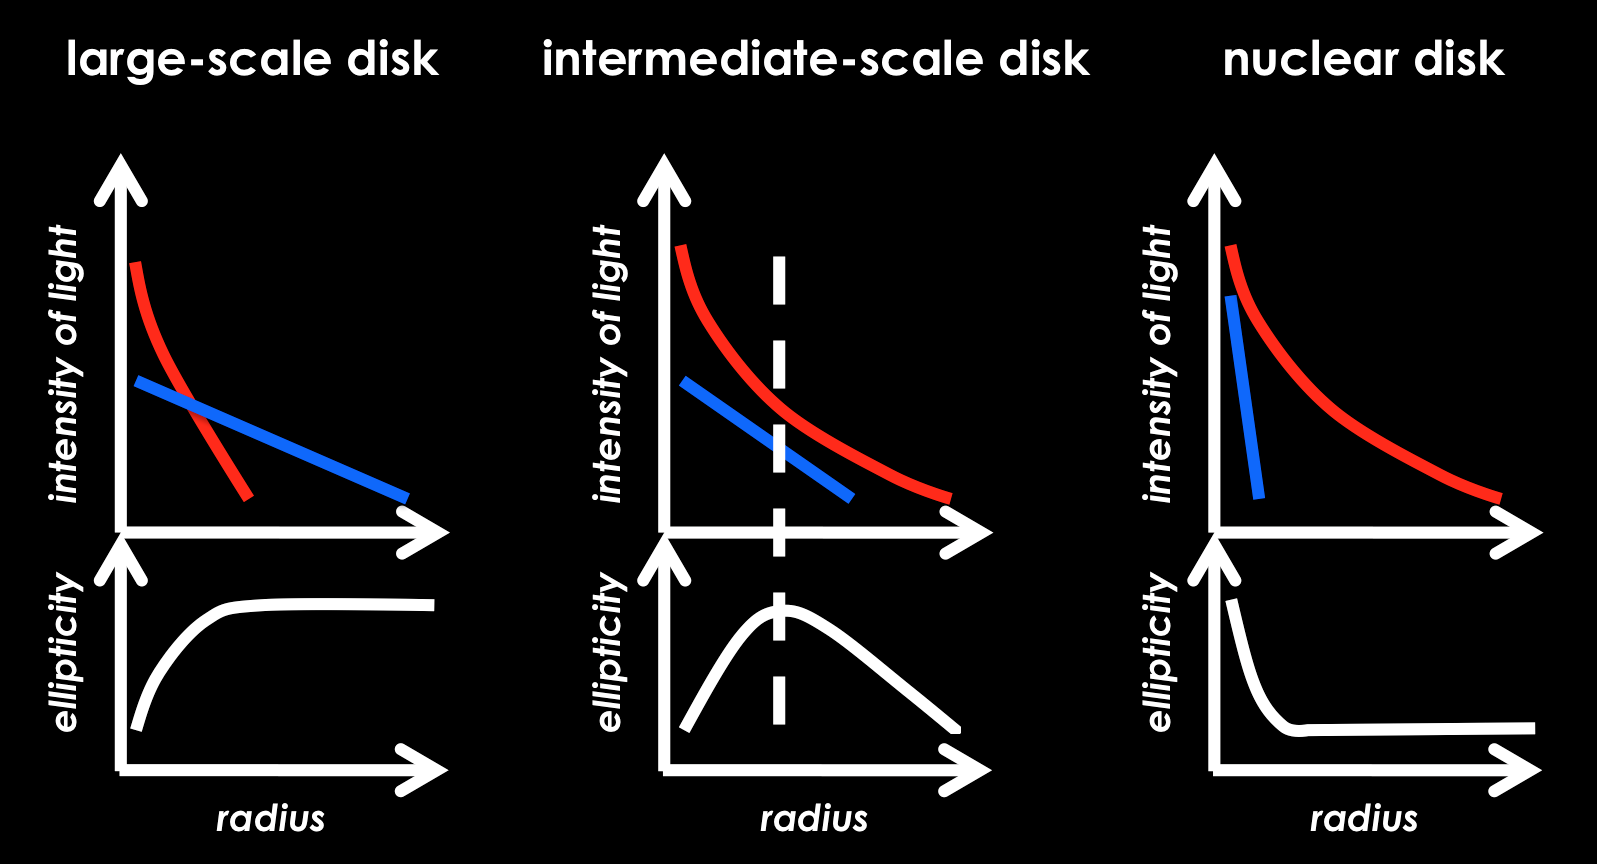
\includegraphics[width=\columnwidth]{images/diskextent.eps}
\caption{Illustration of the typical light profile (top plots) and ellipticity profile (bottom plots) of a galaxy 
featuring a stellar disk with varying size. 
For simplicity, we show separately the light profile of the bulge (or spheroid) in red 
and that of the disk in blue. 
The sum of these two contributions gives the galaxy's light profile (not represented here).
The left panel shows the case of a large-scale disk, {\bf prototipico} of a barless lenticular galaxy. 
The right panel displays the case of an elliptical galaxy with a nuclear stellar disk. 
The middle panel presents the case of a lentiptical galaxy with an inermediate-sized disk. 
Stellar disks typically have fixed ellipticity, dictated by their inclination to our line of sight.
Bulges, instead, can have their ellipticities varying with radius,
but they are usually rounder than inclined disks, 
thus their average ellipticity is lower than that of an inclined disk.
If the ellipticity profile of a galaxy increases with radius, 
this can be ascribed to an inclined disk that becomes progressively more important over the bulge,
whereas a radial decrease of ellipticity signifies the opposite case. 
Therefore the ``shape'' of the ellipticity profile can be decisive to distiguish between 
large- and intermediate-scale disks. 
}
\label{fig:ellp}
\end{figure}

\begin{figure}
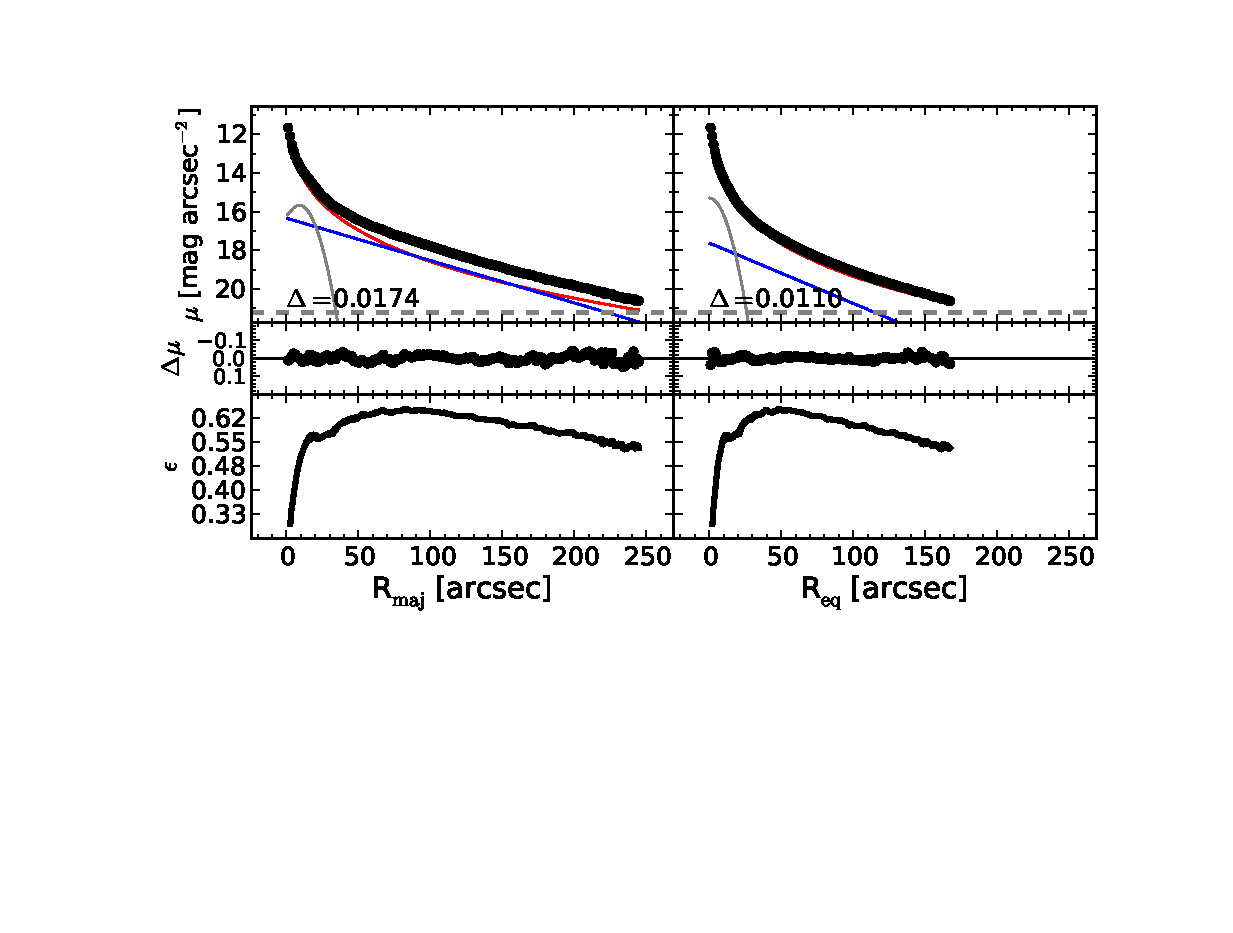
\includegraphics[width=\columnwidth]{images/n3115_decomposition.eps}
\caption{
}
\label{fig:n3115}
\end{figure}

\begin{figure}
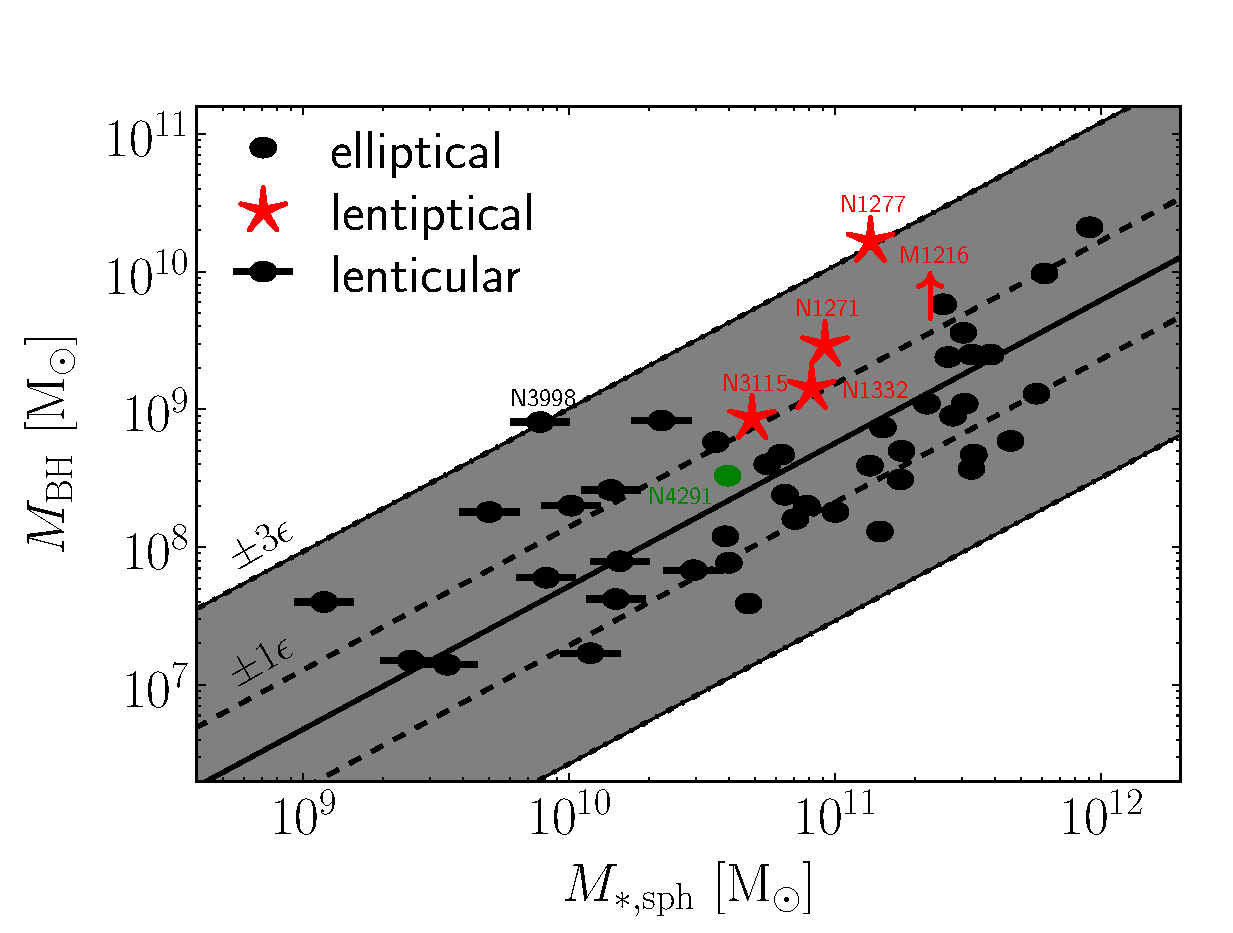
\includegraphics[width=\columnwidth]{images/mm.eps}
\caption{
}
\label{fig:mm}
\end{figure}


%%We are grateful to V. Barger, T. Han, and R. J. N. Phillips for
%%doing the math in section~\ref{bozomath}.
%%More information on the AASTeX macros package is available \\ at
%%\url{http://www.aas.org/publications/aastex}.
%%For technical support, please write to
%%\email{aastex-help@aas.org}.
%%
%%%% To help institutions obtain information on the effectiveness of their
%%%% telescopes, the AAS Journals has created a group of keywords for telescope
%%%% facilities. A common set of keywords will make these types of searches
%%%% significantly easier and more accurate. In addition, they will also be
%%%% useful in linking papers together which utilize the same telescopes
%%%% within the framework of the National Virtual Observatory.
%%%% See the AASTeX Web site at http://aastex.aas.org/
%%%% for information on obtaining the facility keywords.
%%
%%%% After the acknowledgments section, use the following syntax and the
%%%% \facility{} macro to list the keywords of facilities used in the research
%%%% for the paper.  Each keyword will be checked against the master list during
%%%% copy editing.  Individual instruments or configurations can be provided 
%%%% in parentheses, after the keyword, but they will not be verified.
%%
%%{\it Facilities:} \facility{Nickel}, \facility{HST (STIS)}, \facility{CXO (ASIS)}.
%%
%%%% Appendix material should be preceded with a single \appendix command.
%%%% There should be a \section command for each appendix. Mark appendix
%%%% subsections with the same markup you use in the main body of the paper.
%%
%%%% Each Appendix (indicated with \section) will be lettered A, B, C, etc.
%%%% The equation counter will reset when it encounters the \appendix
%%%% command and will number appendix equations (A1), (A2), etc.
%%
%%\appendix
%%
%%\section{Appendix material}
%%
%%Consider once again a task that computes profile parameters for a modified
%%Lorentzian of the form
%%\begin{equation}
%%I = \frac{1}{1 + d_{1}^{P (1 + d_{2} )}}
%%\end{equation}
%%where
%%\begin{mathletters}
%%\begin{displaymath}
%%d_{1} = \frac{3}{4} \sqrt{ \left( \begin{array}{c} \frac{x_{1}}{R_{maj}}
%%\end{array} \right) ^{2} +
%%\left( \begin{array}{c} \frac{y_{1}}{R_{min}} \end{array} \right) ^{2} }
%%\end{displaymath}
%%\begin{equation}
%%d_{2} = \case{3}{4} \sqrt{ \left( \begin{array}{c} \frac{x_{1}}{P R_{maj}}
%%\end{array} \right) ^{2} +
%%\left( \begin{array}{c} \case{y_{1}}{P R_{min}} \end{array} \right) ^{2} }
%%\end{equation}
%%\begin{eqnarray}
%%x_{1} & = & (x - x_{0}) \cos \Theta + (y - y_{0}) \sin \Theta \\
%%y_{1} & = & -(x - x_{0}) \sin \Theta + (y - y_{0}) \cos \Theta
%%\end{eqnarray}
%%\end{mathletters}
%%
%%For completeness, here is one last equation.
%%\begin{equation}
%%e = mc^2
%%\end{equation}

%% The reference list follows the main body and any appendices.
%% Use LaTeX's thebibliography environment to mark up your reference list.
%% Note \begin{thebibliography} is followed by an empty set of
%% curly braces.  If you forget this, LaTeX will generate the error
%% "Perhaps a missing \item?".
%%
%% thebibliography produces citations in the text using \bibitem-\cite
%% cross-referencing. Each reference is preceded by a
%% \bibitem command that defines in curly braces the KEY that corresponds
%% to the KEY in the \cite commands (see the first section above).
%% Make sure that you provide a unique KEY for every \bibitem or else the
%% paper will not LaTeX. The square brackets should contain
%% the citation text that LaTeX will insert in
%% place of the \cite commands.

%% We have used macros to produce journal name abbreviations.
%% AASTeX provides a number of these for the more frequently-cited journals.
%% See the Author Guide for a list of them.

%% Note that the style of the \bibitem labels (in []) is slightly
%% different from previous examples.  The natbib system solves a host
%% of citation expression problems, but it is necessary to clearly
%% delimit the year from the author name used in the citation.
%% See the natbib documentation for more details and options.

%\bibliography{/Users/gsavorgnan/galaxy_vivisection/papers/SMBHbibliography}


\clearpage


\end{document}

%%
%% End of file `sample.tex'.
